% VUT FIT MITAI
% SUR 2019/2020
% Project
% Authors: Vladimir Dusek, David Ling, Richard Mička, Tomáš Strych

%%%%%%%%%%%%%%%%%%%%%%%%%%%%%%%%%%%%%%%%%%%%%%%%%%%%%%%%%%%%%%%%%%%%%

\documentclass{article}

\usepackage[a4paper]{geometry}
\usepackage[utf8]{inputenc}
\usepackage[czech]{babel}
\usepackage{pdfpages}
\usepackage[T1]{fontenc}
\usepackage{amsfonts}
\usepackage{float}
\usepackage[obeyspaces]{url}
\usepackage[bottom]{footmisc}
\usepackage{xcolor}

\newgeometry{left=4.06cm, text={14cm,23.47cm}, top=2.5cm, marginparwidth=50pt}

\restylefloat{table}

\title{Projektová dokumentace \\
    \large Strojové učení a rozpoznávání 2019/2020}
\author{Vladimír Dušek\and David Ling \and Richard Mička \and Tomáš Strych}
\date{\today}

%%%%%%%%%%%%%%%%%%%%%%%%%%%%%%%%%%%%%%%%%%%%%%%%%%%%%%%%%%%%%%%%%%%%%

\begin{document}

\maketitle

%%%%%%%%%%%%%%%%%%%%%%%%%%%%%%%%%%%%%%%%%%%%%%%%%%%%%%%%%%%%%%%%%%%%%

\section{Rozpoznávání obrazu -- Vlastní neuronová síť}

Pro klasifikátor hledané osoby na základě příznaků extrahovaných
z~obrázků byla sestavena a natrénována vlastní neuronová síť.
Byl využit programovací jazyk Python s~frameworkem \texttt{Tensorflow} a nadstavbou \texttt{Keras}.

\subsection{Příprava dat} \label{priprava_dat}

Nejprve bylo nutné připravit data pro trénování.
Poměr trénovacích a validačních dat byl ponechán původní, tak jak byl rozdělen v~zadání.
Pro zpracování dat byl napsán skript \texttt{compile\_data.py}.
Ten nejprve za využití knihovny \texttt{OpenCV} načte obrázky
do reprezentace \texttt{NumPy} \textit{array}.
Tím jsou získány příznaky (\textit{features}) pro trénování.
Každému obrázku je také přiřazena příslušná třída (\textit{label}).
Výsledkem tohoto procesu je dvojice (\textit{feature}, \textit{label})
pro každý trénovací či validační vzorek.
Nakonec jsou pomocí knihovny \texttt{Pickle} uloženy příznaky a označení do binárních souborů
pro trénovací i validační data.\footnote{Je vhodné doplnit,
že tento přístup není úplně vhodný, zejména pro velké datasety.
Všechny obrázky jsou načítány do paměti, to je pochopitelně velmi limitující.
Konkrétně by nebylo možné použít dataset větší, než je velikost operační paměti.
V~našem případě to vzhledem k~malému datasetu není problém, avšak jinak je běžnou praxí
používat Python generátory a data rovnou poskytovat trénovacímu modulu.}

Později se ukázalo, že výsledky trénování nejsou vůbec uspokující.
Bylo vyzkoušeno spoustu nastavení parametrů sítě (více v~sekci \ref{trenovani}),
avšak se nedařilo dosáhnout žádného výrazného zlepšení.
Z~toho bylo vyvozeno, že je k~dispozici příliš málo trénovacích dat
a síť se na nich není schopná nic rozumného naučit.
Typický průběh trénování byl takový, že po prvních několika málo epochách již
na validačních datech nedocházelo k~žádnému zlepšení.

Z~toho důvodu byla vyzkoušena technika augmentace dat.
Pomocí jednoduchého Python nástroje imgaug (dostupný na \path{github.com/aleju/imgaug})
bylo základními úpravami dosaženo vytvoření nových dat.
Byly použity úpravy jako zrcadlové otočení, přidání rozmazání, přidání šumu
či mírné natočení obrazu.
Na takto augmentovaných datech poté probíhalo další trénování a bylo dosaženo
značně lepších výsledků.

\subsection{Trénování} \label{trenovani}

Pro trénování modelů byl napsán skript \texttt{train\_models.py}.
Nejprve jsou pomocí knihovny \texttt{Pickle} načteny již připravená trénovací data.
Následně jsou příznaky normalizovány vydělením maximem.
Tím je dosaženo toho, že každá hodnota reprezentující pixel je přeškálována
do intervalu $(0,1)$.
Dalším krokem je, vzhledem k~nerovnoměrnému rozložení trénovacích dat
pro třídu \textit{target} a \textit{nontarget}, spočítat jejich poměr.
Při trénování sítě je tento poměr zohledňován, a díky tomu síť uvažuje,
že je každá třída stejně pravděpodobná.
Dále je při trénování využit plugin \texttt{TensorBoard},
který ukládá logy z~trénování (chyby a přesnosti na trénovacích/validačních datech).

Byly vyzkoušeny různé konfigurace neuronových sítí a celkem bylo natrénováno 108 modelů.
Konkrétně počet konvolučních vrstev 1, 2 a 3.
Velikost konvolučních jader 32, 64 a 128 neuronů.
Konvoluční vrstvy následované \textit{dropout} vrstvou.
Počet plně propojených vrstev 0, 1 a 2.
Počet neuronů v~plně propojené vrstvě 256 a 512.
Všechny vrstvy obsahují aktivační funkci ReLU (\textit{Rectified Linear Unit}).
Pouze výstupní plně propojená vrstva o~jednom neuronu má aktivační funkci \textit{sigmoid},
aby skóre pro jednotlivé třídy bylo naškálováno do intervalu $(0,1)$.
Tím je získána pravděpodobnost náležitosti konkrétním třídám.

Na augmentovaných datech byly postupně všechny modely trénovány 15 epoch.
Jako nejúspěšnějsí se ukázal model s~jednou konvoluční vrstvou o~velikosti 128 neuronů,
následovanou \textit{max pooling} vrstvou, \textit{dropout} vrstvou s~pravdědpobností $0,35$
a dvěma plně propojenými vrstvami s~512 neurony.
Konkrétně po 10. epoše bylo dosáhnuto nejvyšší přesnosti na validačních datech 92\,\%
(viz obrázek~\ref{vyvoj_presnosti}).

\begin{figure}[H]
    \centering
    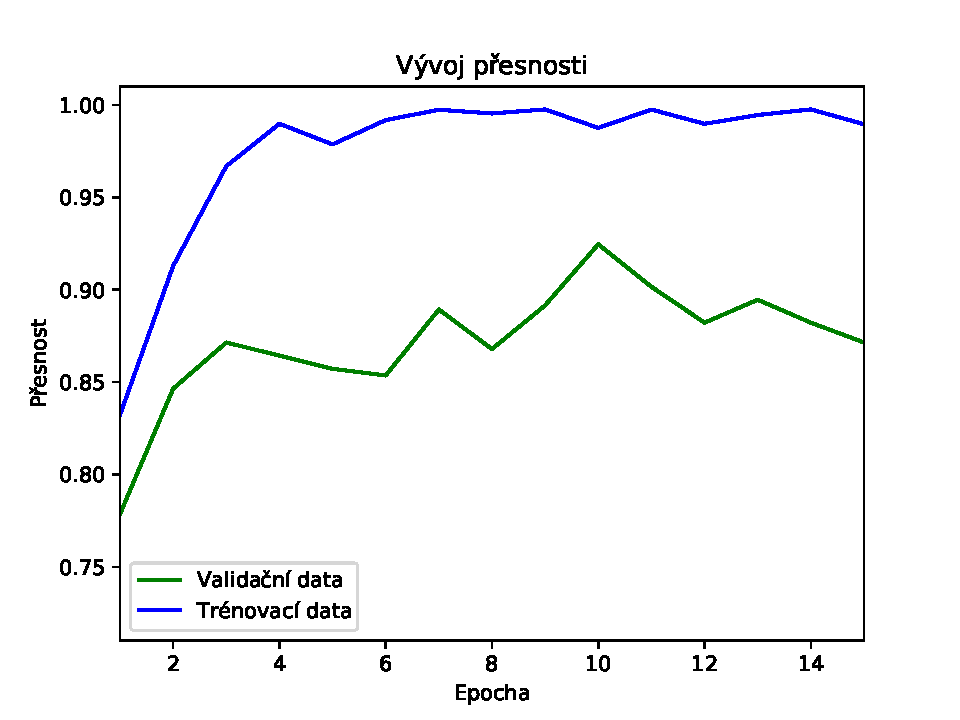
\includegraphics[width=.75\textwidth]{img/acc-plt.pdf}
    \caption{Vývoj přesnosti v~průběhu testování.}
    \label{vyvoj_presnosti}
\end{figure}

\subsection{Vyhodnocení} \label{evaluace}

Pro vyhodnocení evaluačních dat byl napsán skript \texttt{eval.py}.
Ten načte příslušný natrénovaný model a pomocí knihovny \texttt{os} na něm spustí detekci
pro všechna evaluační data.
Generuje výstupní soubor \texttt{out.txt}, do kterého zapisuje požadované informace,
tedy jméno vzorku, skóre a výslednou třídu.

%%%%%%%%%%%%%%%%%%%%%%%%%%%%%%%%%%%%%%%%%%%%%%%%%%%%%%%%%%%%%%%%%%%%%

\section{Rozpoznávanie obrazu - predtrénovaná sieť}
Našim cieľom bolo dosiahnuť čo najlepších výsledkov za čo najmenej času. Preto sme sa rozhodli použiť predtrénované modely. Zvolili sme použitie modelu Resnet50. Vybrané boli dva modely, z ktorých jeden bol predtrénovaný na datasete VGGFace2\footnote{VGGFace2 - \url{http://www.robots.ox.ac.uk/~vgg/data/vgg_face2/}}, ktorý pozostáva z približne troch miliónov obrazov tváre a samotný model bol natrénovaný na klasifikáciu približne osem tisíc tried obrazov, a druhý na bol predtrénovaný na datasete ImageNet\footnote{ImageNet - \url{http://image-net.org/}}, ktorý pozostáva zo 14 miliónov obrázkov s približne 20 tisícami kategórií na klasifikáciu. Avšak v~prípade ImageNet to nie sú exkluzívne obrazy ľudských tvárí. Ako prebiehalo trénovanie modelu ResNet50\footnote{ResNet50 - \url{https://arxiv.org/abs/1512.03385}} predtrénovanom na datasete VGGFace2 je popísané v nasledujúcej podkapitole. Následne bude popísaná sieť ResNet50 s datasetom ImageNet, ktorý obsahuje rôzne kategórie obrázkov. Obidve predtrénované siete boli trénované pomocou nástroja \texttt{Google Colab} a využívajú knižnicu \texttt{PyTorch}.

\subsection{ResNet50 s datasetom VGGFace2}
Táto sieť pripadá ako vhodná voľba za účelom jednoduchej a pritom vysoko spoľahlivej klasifikácie tvárí, pretože ide o veľmi úspešnú architektúru hlbokej konvolučnej siete na klasifikáciu obrázkov ResNet, ktorá je špeciálne trénovaná na sade obrazov tvárí. Na základe toho sa dá predpokladať dobrá prenositeľnosť naučených váh aj na dátovú sadu dostupnú v rámci tohto projektu. Táto predtrénovaná sieť je trénovaná na klasifikáciu plibližne 8000 rôznych tried klasifikácie -- ľudských tvárí.

Bežný vstup tejto siete má rozmery 3x224x224 (kanály, výška, šírka), čo nesedí s rozmermi dátovej sady projektu. Preto boli pred použitím tohto modelu potrebné kroky, ktorými bolo umožnené jeho požitie. Išlo o zmenu kroku (stride) prvej konvolučnej vrstvy pôvodného modelu z 2 na 1. Týmto krokom sa nezmenia predtrénované váhy konvolučných filtrov prvej vrstvy, pretože rozmery filtra sa nemenia, avšak má to za následok zmenu rozmerov výstupu tejto vrstvy. Zmenšením kroku filtra sa šírka a výška výstupu zdvojnásobí. To zaručí, že pri vložení ako vstupu obrázku s polovičnými rozmermi šírky a výšky, budú rozmery výstupu tejto vrstvy rovnakých rozmerov, ako pri pôvodnom kroku filtra v prvej vrstve a pôvodných rozmeroch obrazu. Týmto sa zmenšili rozmery vstupu modelu na veľkosť 3x112x112. Keďže rozmery obrazov boli 3x80x80, tento krok samotný nepostačuje a tak bolo potrebné všetky obrazy pri nahratí zväčšiť na rozmery 3x112x112. Zväčšovanie bolo realizované knižnicou \texttt{PIL} pomocou bilineárneho filtra počas nahrávania datovej sady. Posledným potrebným krokom bolo odčítanie stredných hodnôt jednotlivých kanálov trénovacej sady. Tieto parametre sú súčasťou predtrénovaného modelu.

Na samotnú klasifikáciu bol použitý výstup predposlednej vrstvy realizujúcej \texttt{average pooling} s výstupným vektorom o rozmere 2048 features, na ktorý bola pripojená a dotrénovaná lineárna vrstva s 2 výstupmi a funkciou \texttt{Softmax} medzi nimi. V~pôvodnom predtrénovanom modeli bola posledná vrstva realizovaná obdobne na počet tried 8631 pomocou 1x1 konvolúcie (ktorá je ekvivalentná s lineárnou vrstvou). Počas trénovania boli upravované váhy len nami dodanej vrstvy a váhy predchádzajúcich vrstiev boli ponechané na pôvodných hodnotách z~predtrénovaného modelu.

V~rámci pokusu o použitie predtrénovaných modelov na sade VGGFace2 bol taktiež realizovaný pokus o použitie menšieho modelu Squzee-Excitation ResNet50 `SE-ResNet-50-128D` natrénovaného do embedujúceho 128-dimenzionálneho feature priestoru. Tento model však nebolo triviálne natrénovať na nám dostupnej trénovacej sade a vyžadoval by si väčšiu prácu, či už v nastavení a ladení parametrov pripojených výstupných vrstiev, alebo nastavovaní trénovacích parametrov a úprave datasetu. Z~dôvodu jednoduchosti aplikácie pôvodného modelu ResNet 50 a jeho vynikajúcej schopnosti klasifikácie však neboli realizované ďalšie pokusy s použitím tohto menšieho modelu.

\subsection{ResNet50 s datasetom ImageNet}
Ideou bolo otestovať, či sa model naučený na rozpoznávaní rôznych kategórií obrázkov je schopný naučiť správne rozpoznávať tváre.\\

V tomto prípade bola poskytnutým obrázkom zmenená veľkosť na 3x250x250. Potom bol vystrihnutý stred obrázkov na rozmer 3x224x224. Po normalizácii dát tak mala sieť pripravené dáta k trénovaniu.

Cieľom siete je aby rozoznávala, azda sa na obrázku nachádza osoba, ktorú hľadamé alebo nie. Preto bola posledná vrstva pozmenená na lineárnu s 2 výstupmi. Okrem toho boli zmrazené váhy v celej sieti okrem poslednej vrstvy. Táto posledná vrstva má pred trénovaním náhodne generované váhy. Bola použitá CrossEntropyLoss funkcia.

Takto upravená sieť bola natrénovaná a vyhodnotená. Aby sme pri vyhodnocovaní získali pravdepodobnosti tak výstupi siete boli prepočítané cez softmax. Jednoduchým python skriptovaním bolo na evaluačnej sade vyhodnotené, koľko obrázkov bolo špecifikovaných správne a koľko nie. Pri nesprávne špecifikovaných obrázkoch pre jednotlivé kategórie sú zobrazené názvy obrázkov, čo umožňuje jednoduchšiu investigáciu toho prečo sa modelu nedarilo tieto obrázky správne rozoznať.

%%%%%%%%%%%%%%%%%%%%%%%%%%%%%%%%%%%%%%%%%%%%%%%%%%%%%%%%%%%%%%%%%%%%%

\section{Rozpoznávání zvuku}

\subsection{Popis vybraných klasifikačních metod}
Jako klasifikátor pro zvukové nahrávky byl použit gaussovský klasifikátor založený na směsici gaussovských rozložení (anglicky Gaussian Mixture Model, zkratkou GMM).\\
Tento algoritmu byl vybrán z důvodu toho, že dobře generalizuje i na neviděná data a jednoduché implementace. Algoritmus se snaží odhadnout co nejlépe parametry $n$ gaussovských rozložení pro trénovací data a poté nově přichozí data klasifikovat do jedné z $c$ tříd.\\
Pro trénink klasifikátoru byla vybrána metoda Expectation maximization, která pracuje tak, že se snaží nalézt takové parametry (střední hodnota a kovarianční matice) GMM, aby hodnota funkce $L$ vracející věrohodnost dat, byla maximální.\\

\subsection{Popis implementace a volba parametrů}
Implementace byla provedena v jazyce Python za využití funkcí z knihovny \texttt{ikrlib}.\\
Všechna trénovací data se před spuštěním vložila do složky \texttt{data/train/číslo\_třídy}, takže data pro hledanou osobu byly ve složce \texttt{data/train/1} a ostatní ve složce \texttt{data/train/2}. Data pro klasifikaci poté všechna do složky \texttt{data/eval}. Apriorní prvděpodobnost byla spočítána pro jednotlivé třídy na základě počtu trénovacích dat v obou třídách.\\
Po poslechnutí několika nahrávek bylo rozhodnuto, že káždá nahrávka bude oříznuta tak, aby neobsahovala počáteční a koncové ticho, které klasifikaci jednotlivých osob neprospěje. Z každé nahrávky tedy bylo odstraněno prvních 100 a posledních 300 vzorků, což výrazně zvýšilo úspěšnost klasifikátoru.\\
Bylo třeba rozhodnout, jaké parametry zvolit pro trénování klasifikátoru. Jedná se se o:
\begin{itemize}
    \item Počet gaussovských rozložení
    \item Počet iterací trénování pomocí funkce \texttt{train\_gmm}
\end{itemize}

Po testování s různými parametry vyšly jako nejlepší hodnoty 8 pro počet gaussovských rozložení a 110 pro počet iterací trénování.\\
Po natrénování byla pro všechna evaluační data spočtena pravděpodobnost pro obě třídy pomocí funkce \texttt{logpdf\_gmm} a vybraná ta s vyšší pravděpodobností.

%%%%%%%%%%%%%%%%%%%%%%%%%%%%%%%%%%%%%%%%%%%%%%%%%%%%%%%%%%%%%%%%%%%%%

\section{Výsledky}

Nejlépších výsledků dosáhla předtrénovaná síť ResNet50 na datasetu VGGFace, která dosáhla dokonce nulové chybovosti. Také rozpoznávání z řečových nahrávek skončilo výsledkem s chybou v nízkých jednotkách procent. Kompletní výsledky lze vidět v tabulce níže.\\

\centering
\begin{tabular}{ |c|c|c|c|c|  }
 \hline
 \multicolumn{5}{|c|}{Výsledky projektu} \\
 \hline
 Název klasifikátoru & Error & Cdet &  minCdet & EER \\
 \hline
 cnn   & 11.31 & 12.97 & 12.89 & 15.02\\
 gmm\_speech & 2.53 & 1.39 & 0.65 & 1.49\\
 resnet50\_finetuned\_result & 4.91 & 17.73 & 17.40 & 21.86\\
 resnet50\_vggface2\_pretrained & 0.00 & 0.00 & 0.00 & 0.00\\
 \hline
\end{tabular}

%%%%%%%%%%%%%%%%%%%%%%%%%%%%%%%%%%%%%%%%%%%%%%%%%%%%%%%%%%%%%%%%%%%%%

\end{document}
